\documentclass[11pt,a4paper]{article}
\usepackage[utf8]{inputenc}
\usepackage{color}
\usepackage{enumerate}
\usepackage{fancyhdr}
\usepackage{minted}
\usepackage{graphicx}
\usepackage{array}
\usepackage{hyperref}
\usepackage{amssymb}
\usepackage{multirow}
\usepackage[spanish]{babel}
\usepackage[spanish]{algorithm2e}

\setlength{\oddsidemargin}{18pt}
\setlength{\headheight}{14pt}
\setlength{\textheight}{619pt}
\setlength{\marginparsep}{11pt}
\setlength{\footskip}{30pt}
\hoffset = 0pt
\voffset = 0pt
\setlength{\topmargin}{0pt}
\setlength{\headsep}{25pt}
\setlength{\textwidth}{424pt}
\setlength{\marginparwidth}{54pt}
\setlength{\marginparpush}{5pt}
\paperwidth = 597pt
\paperheight = 845pt

\pagestyle{fancy}
\fancyhead[LO]{\textcolor[rgb]{0,0,0}{Grado en Ingeniería Informática}}
\fancyhead[RO]{\textcolor[rgb]{0.2,0.2,0.9}{Algorítmica, Curso 2015-2016}}

\hypersetup{
	colorlinks,
	citecolor=black,
	filecolor=black,
	linkcolor=black,
	urlcolor=black
}

\begin{document}

	\begin{titlepage}

		\centering

		\begin{figure}[h]

			\centering
			
\includegraphics[width=0.6\textwidth]{logo-ugr.png}
			
		\end{figure}

		\vspace{1cm}

		{\scshape\LARGE Universidad de Granada}

		\vspace{1cm}

		{\LARGE Algorítmica}

		\vspace{1cm}

		{\huge\bfseries\textit{Algoritmos Backtracking y Ramificación y Poda, parte 2}}

		\vspace{1cm}

		{\itshape\large 
		Laura Calle Caraballo \\
		Cristina María Garrido López \\
		Germán González Almagro \\
		Javier León Palomares \\
		Antonio Manuel Milán Jiménez}

		\vfill

		{\Large\today}

	\end{titlepage}

\newpage

	\tableofcontents

\newpage

	\section{Introducción.}

		\par
		El objetivo de esta práctica es el estudio de las técnicas de tipo \textit{Ramificación y Poda} y \textit{Backtracking}, aplicadas particularmente al problema del viajante de comercio. Para ello, hemos implementado ambos algoritmos y, adicionalmente, hemos probado algunas modificaciones sobre el primero de ellos.

	\section{Descripción del problema.}

		\par
		El problema del viajante de comercio, también llamado \textit{TSP} por sus siglas en inglés, es conocido desde el siglo XIX y fue planteado en su forma general en la década de 1930; desde entonces, es uno de los problemas más estudiados en optimización. Su complejidad hace computacionalmente muy costosa una solución mediante fuerza bruta. Por ello, se han ido creando una serie de métodos que obtienen resultados válidos según la situación: soluciones exactas para dimensiones pequeñas, aproximadas para dimensiones más grandes o particularizaciones del problema donde se pueda emplear una aproximación mejor.

		\par
		La pregunta que busca responder este problema es la siguiente: \textit{``Considerando un conjunto de ciudades y las distancias entre ellas dos a dos, ¿cuál es el camino más corto que pasa por todas ellas una única vez y retorna al origen?''}

		\par
		En términos de grafos esto significa que, a partir de un grafo ponderado, conexo y no dirigido, debemos encontrar el circuito hamiltoniano de menor peso.

	\section{Resolución.}

		\par
		Para afrontar la resolución de este problema de forma exacta, hemos implementado un algoritmo de \textit{Ramificación y Poda}, también denominado \textit{Branch and Bound}. Las características de esta técnica particularizadas para el problema del viajante de comercio son las siguientes:

		\begin{itemize}

			\item
			Solución: vector que contiene todas las ciudades de la instancia a evaluar ordenadas según se recorren para formar un circuito hamiltoniano.
			\item
			Función de poda: si una solución parcial tiene una cota inferior mayor que el coste de la mejor solución encontrada hasta el momento (cota superior), se realiza una poda.
			\item
			Restricciones explícitas: las ciudades almacenadas en la solución pertenecen a la instancia que se está evaluando.
			\item
			Restricciones implícitas: una ciudad no puede aparecer más de una vez en la solución (excepto si representamos el cierre del circuito añadiendo de nuevo la ciudad de partida).
			\item
			Espacio de soluciones: las permutaciones de tamaño $n$, siendo $n$ la dimensión del problema.

		\end{itemize}

		\par
		Según lo anterior, es necesario el uso de dos tipos de cotas: una superior y una inferior. La cota superior representa el coste de la mejor solución conocida por el algoritmo, y será global. La cota inferior se define para cada solución parcial, y representa el coste desde el inicio hasta la última ciudad insertada sumado a una estimación optimista del costo restante. Usando estos valores podemos podar cuando la cota inferior de una solución parcial sea mayor que la cota superior, ya que significa que dicha solución parcial nunca podrá ser mejor que lo que ya tenemos.

		\par
		Adicionalmente, se ha implementado un algoritmo \textit{Backtracking} que también consta de los elementos antes listados.

		\subsection{Algoritmo de \textit{Ramificación y Poda}.}

			\subsubsection{Pseudocódigo.}

				\par
				A continuación, explicamos el funcionamiento de esta técnica mediante pseudocódigo:

				\vspace{2mm}

				\begin{algorithm}[H]

					\textbf{function} ViajanteComercio(conjuntoCiudades,ciudadInicial);

					mejorCoste $\longleftarrow$ cotaSuperior\footnotemark[1]\;
					caminoInicial $\longleftarrow$ ciudadInicial\;
					abiertos.push(caminoInicial)\;

					\Begin{

						\While{abiertos \textbf{not} empty}{

							caminoActual $\longleftarrow$ abiertos.top()\;
							abiertos.pop()\;

							\uIf{EsSolucion(caminoActual)}{

								\If{Coste(caminoActual)\footnotemark[2] $<$ mejorCoste}{

									mejorCamino $\longleftarrow$ caminoActual\;
									mejorCoste $\longleftarrow$ Coste(caminoActual)\;

								}
							}

							\ElseIf{Valoracion(caminoActual) $<$ mejorCoste}{

								\While{quedan hijos sin generar}{

									hijo $\longleftarrow$ GeneraHijo(caminoActual)\;

									\If{Valoracion(hijo) $<$ mejorCoste}{

										abiertos.push(hijo)\;

									}
								}
							}
						}

						\KwRet mejorCamino, mejorCoste\;

					}

				\end{algorithm}

				\vfill

				\footnotetext[1]{La cota superior inicial puede tomar el valor $\infty$ o bien el resultado de un algoritmo \textit{Greedy}.}
				\footnotetext[2]{Nótese la diferencia entre las funciones \textit{Coste(camino)} y \textit{Valoracion(camino)}. La primera es usada para caminos completos y no contiene elementos heurísticos; en cambio, la segunda se utiliza para caminos parciales y siempre tiene una componente de estimación de coste. Esto es aplicable también a la siguiente sección.}

	\newpage

		\subsection{Algoritmo \textit{Backtracking}.}

			\par
			A diferencia de la técnica de \textit{Ramificación y Poda}, \textit{Backtracking} no prioriza su exploración por criterios de coste o heurísticos, sino que explora cada rama en profundidad. Sin embargo, podemos reducir la búsqueda introduciendo la función de poda que hemos usado anteriormente.

			\subsubsection{Pseudocódigo.}

				\par
				A continuación se muestra el pseudocódigo del algoritmo incluyendo la función de poda:

				\vspace{2mm}

				\begin{algorithm}[H]

					ciudadActual $\longleftarrow$ ciudadInicial\;
					caminoActual $\longleftarrow$ caminoActual $\cup$ ciudadActual\;
					mejorCoste $\longleftarrow$ cotaSuperior\;

					\textbf{function} ViajanteComercio(conjuntoCiudades, caminoActual);

					\Begin{

						\uIf{EsSolucion(caminoActual)}{

							\If{Coste(caminoActual) $<$ mejorCoste}{

								mejorCamino $\longleftarrow$ caminoActual\;
								mejorCoste $\longleftarrow$ Coste(caminoActual)\;

							}
						}

						\ElseIf{Valoracion(caminoActual) $<$ mejorCoste}{

							\While{quedan hijos sin generar}{

								hijo $\longleftarrow$ GeneraHijo(caminoActual)\;

								caminoActual $\longleftarrow$ caminoActual $\cup$ hijo\;

								ViajanteComercio(conjuntoCiudades,caminoActual)\;

							}
						}

						caminoActual $\longleftarrow$ caminoActual $-$ caminoActual.back()\;

					}

				\end{algorithm}

\newpage

	\hypertarget{improvements}{\section{Mejoras sobre el algoritmo de \textit{Ramificación y Poda}.}}

		\par
		En esta sección analizaremos cómo el nivel de optimización al compilar y ciertos cambios en las cotas superiores e inferiores afectan al rendimiento de esta técnica.

		\subsection{Optimización en tiempo de compilación.}

			\par
			Todas las mediciones incluidas en esta memoria han sido realizadas con el nivel de compilación 2 del compilador \textit{g++}. Una muestra de la diferencia con una compilación normal se puede ver en la siguiente tabla:

			\begin{figure}[h]

				\centering

				\begin{tabular}{| >{\centering\arraybackslash}m{1in} | >{\centering\arraybackslash}m{1in} | >{\centering\arraybackslash}m{1in} |}

					\hline
					\textbf{Tamaño} & \textbf{Nivel 0} & \textbf{Nivel 2} \\
					\hline
					9 & 0.066694 & 0.005936 \\
					\hline
					11 & 1.0335 & 0.097976 \\ 
					\hline
					13 & 25.5159 & 2.39737 \\
					\hline
					15 & 1192.46 & 113.248 \\
					\hline 

				\end{tabular}
				\caption{Tiempos de ejecución de \textit{Ramificación y Poda} con optimizaciones 0 y 2.}

			\end{figure}

		\subsection{Cota inferior (heurística).}

			\par
			Hemos probado dos heurísticas diferentes, una menos costosa pero menos precisa (heurística 1) y otra más costosa pero más precisa (heurística 2):

			\begin{itemize}

				\item
				Heurística 1: la valoración de un nodo consiste en el coste real desde el inicio hasta la última ciudad añadida más la suma de la distancia más corta asociada a cada ciudad no contenida en el circuito.
				\item
				Heurística 2: similar a la anterior, pero sustituyendo cada distancia más corta asociada a cada ciudad no incluida por la media de las dos distancias más cortas.

			\end{itemize}

			\par
			Aquí tenemos una tabla comparando los tiempos de ejecución obtenidos:

			\vspace{2mm}

			\begin{figure}[h]

				\centering

				\begin{tabular}{| >{\centering\arraybackslash}m{1in} | >{\centering\arraybackslash}m{1in} | >{\centering\arraybackslash}m{1in} |}

					\hline
					\textbf{Tamaño} & \textbf{Heurística 1} & \textbf{Heurística 2} \\
					\hline
					9 & 0.005936 & 0.010186 \\
					\hline
					10 & 0.025171 & 0.021891 \\
					\hline
					11 & 0.097976 & 0.150797 \\ 
					\hline
					12 & 0.40271 & 0.327216 \\
					\hline
					13 & 2.39737 & 1.88105 \\
					\hline
					14 & 15.5334 & 13.411 \\
					\hline
					15 & 113.248 & 76.734 \\
					\hline
					16 & 507.988 & 475.295 \\
					\hline 
					17 & 1403.64 & 1342.11 \\
					\hline

				\end{tabular}
				\caption{Tiempos de ejecución del algoritmo de \textit{Ramificación y Poda} con las dos heurísticas sobre subconjuntos de la instancia \textit{ulysses22}.}

			\end{figure}

\newpage

			\par
			La gráfica de tiempos de ejecución es la siguiente:

			\vspace{2mm}

			\begin{figure}[h]

				\centering
				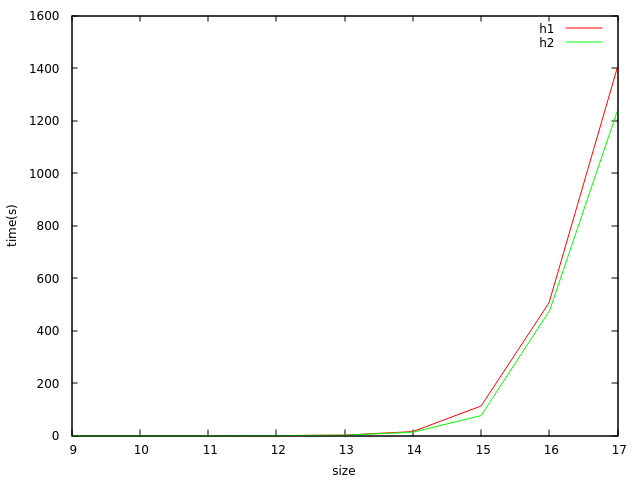
\includegraphics[width=0.75\textwidth]{ComparativaH1-H2.png}
				\caption{Gráfica comparativa de tiempos de ejecución. Intel® Core™ i5-5200U CPU @ 2.20GHz.}
				
			\end{figure}

			\vspace{2mm}

			\par
			Además, podemos observar diferencias en el número de nodos expandidos, el número de podas realizadas y el tamaño máximo de la lista de nodos abiertos:

			\vspace{2mm}

			\begin{figure}[h]

				\centering

				\resizebox{\textwidth}{!}{
				\begin{tabular}{| >{\centering\arraybackslash}m{1in} | >{\centering\arraybackslash}m{1in} | >{\centering\arraybackslash}m{1in} | >{\centering\arraybackslash}m{1in} | >{\centering\arraybackslash}m{1in} | >{\centering\arraybackslash}m{1in} | >{\centering\arraybackslash}m{1in} |}

					\hline
					\multirow{2}{*}{\textbf{Tamaño}} & \multicolumn{2}{ c |}{Nodos explorados} & \multicolumn{2}{c |}{Podas realizadas} & \multicolumn{2}{c |}{Tamaño máximo de abiertos} \\
					\cline{2-7}
					 & \textbf{Heurística 1} & \textbf{Heurística 2} & \textbf{Heurística 1} & \textbf{Heurística 2} & \textbf{Heurística 1} & \textbf{Heurística 2} \\
					 \hline
					9 & 11835 & 9318 & 13931 & 11037 & 20 & 20 \\
					\hline
					10 & 46104 & 35096 & 68824 & 50800 & 25 & 25 \\
					\hline
					11 & 169904 & 123479 & 315454 & 216650 & 28 & 42 \\ 
					\hline
					12 & 658812 & 501201 & 1411538 & 996808 & 32 & 49 \\
					\hline
					13 & 3700596 & 2664686 & 8897596 & 5897746 & 40 & 98 \\
					\hline
					14 & 22759953 & 17305665 & 59114136 & 40576941 & 46 & 281 \\
					\hline
					15 & 159973208 & 98810551 & 433414136 & 246071382 & 52 & 525 \\
					\hline
					16 & 747710543 & 577997680 & 2075155499 & 1563321736 & 62 & 579 \\
					\hline 
					17 & 2362464162 & 1744774322 & 6545043838 & 5062870607 & 62 & 709 \\
					\hline

				\end{tabular}}
				\caption{Otros datos relevantes de las dos heurísticas.}

			\end{figure}

			\par
			Como apunte, la cota superior inicial utilizada corresponde a una ejecución \textit{Greedy}.

\newpage

			\par
			Como muestra de las diferencias, a continuación mostramos una gráfica con la cantidad de nodos explorados y otra con la cantidad de podas realizadas usando cada heurística:

			\vspace{2mm}

			\begin{figure}[h]

				\centering
				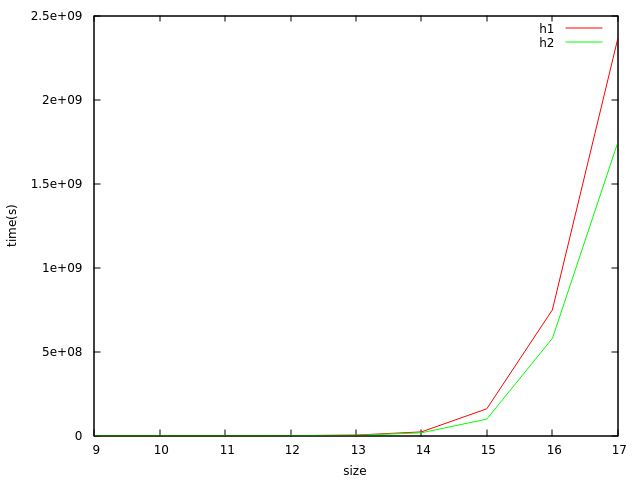
\includegraphics[width=0.64\textwidth]{ComparativaExploradosH1-H2.png}
				\caption{Gráfica comparativa de nodos explorados.}
				
			\end{figure}

			%\vspace{2mm}

			\begin{figure}[h]

				\centering
				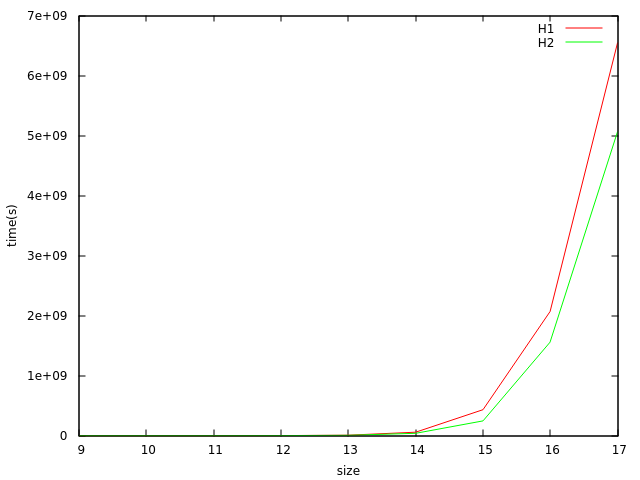
\includegraphics[width=0.64\textwidth]{ComparativaPodadosH1-H2.png}
				\caption{Gráfica comparativa de nodos podados.}
				
			\end{figure}

			\par
			Podemos intuir que, gracias a la mayor precisión de la heurística 2, el algoritmo es capaz de realizar más podas en las fases iniciales, disminuyendo tanto el número total de nodos explorados como el de podas, ya que el factor de ramificación se reduce ligeramente.

\newpage

		\subsection{Cota superior inicial.}

			\par
			Con el objetivo de reducir el espacio de soluciones desde el inicio, podemos acotar el coste máximo que aceptaremos para que sea estrictamente menor que el resultado de un algoritmo \textit{Greedy} frente a una cota inicial con valor infinito. De esta forma, es posible evitar la comprobación de más permutaciones potencialmente inútiles.

			\par
			Veamos primero los tiempos de ejecución:

			\vspace{2mm}

			\begin{figure}[h]

				\centering

				\begin{tabular}{| >{\centering\arraybackslash}m{1in} | >{\centering\arraybackslash}m{1in} | >{\centering\arraybackslash}m{1in} |}

					\hline
					\textbf{Tamaño} & \textbf{Infinito} & \textbf{\textit{Greedy}} \\
					\hline
					9 & 0.006572 & 0.005936 \\
					\hline
					10 & 0.030662 & 0.025171 \\
					\hline
					11 & 0.11359 & 0.097976 \\ 
					\hline
					12 & 0.524846 & 0.40271 \\
					\hline
					13 & 3.01591 & 2.39737 \\
					\hline
					14 & 20.2228 & 15.5334 \\
					\hline
					15 & 142.716 & 113.248 \\
					\hline
					16 & 596.025 & 507.988 \\
					\hline 
					17 & 1510.34 & 1403.64 \\
					\hline

				\end{tabular}
				\caption{Tiempos de ejecución de los dos algoritmos sobre subconjuntos de la instancia \textit{ulysses22}.}

			\end{figure}

			\par
			La gráfica asociada a la tabla anterior es:

			\vspace{2mm}

			\begin{figure}[h]

				\centering
				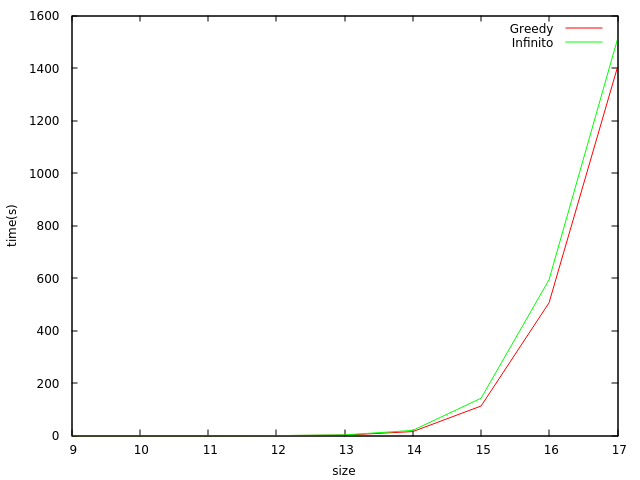
\includegraphics[width=0.75\textwidth]{ComparativaGreedy-Inf.png}
				\caption{Gráfica comparativa de tiempos de ejecución. Intel® Core™ i5-5200U CPU @ 2.20GHz.}
				
			\end{figure}

\newpage

			\par
			Asimismo, los efectos de esta modificación en otros aspectos importantes se pueden observar en la siguiente tabla:

			\vspace{2mm}

			\begin{figure}[h]

				\centering

				\resizebox{\textwidth}{!}{
				\begin{tabular}{| >{\centering\arraybackslash}m{1in} | >{\centering\arraybackslash}m{1in} | >{\centering\arraybackslash}m{1in} | >{\centering\arraybackslash}m{1in} | >{\centering\arraybackslash}m{1in} | >{\centering\arraybackslash}m{1in} | >{\centering\arraybackslash}m{1in} |}

					\hline
					\multirow{2}{*}{\textbf{Tamaño}} & \multicolumn{2}{ c |}{Nodos explorados} & \multicolumn{2}{c |}{Podas realizadas} & \multicolumn{2}{c |}{Tamaño máximo de abiertos} \\
					\cline{2-7}
					 & \textbf{Infinito} & \textbf{\textit{Greedy}} & \textbf{Infinito} & \textbf{\textit{Greedy}} & \textbf{Infinito} & \textbf{\textit{Greedy}} \\
					\hline
					9 & 14620 & 11835 & 16127 & 13931 & 29 & 20 \\
					\hline
					10 & 55346 & 46104 & 77266 & 68824 & 37 & 25 \\
					\hline
					11 & 211088 & 169904 & 369805 & 315454 & 46 & 28 \\ 
					\hline
					12 & 917049 & 658812 & 1859356 & 1411538 & 56 & 32 \\
					\hline
					13 & 4898698 & 3700596 & 11313246 & 8897596 & 68 & 40 \\
					\hline
					14 & 30180661 & 22759953 & 75441404 & 59114136 & 81 & 46 \\
					\hline
					15 & 305703379 & 159973208 & 547508027 & 433414136 & 94 & 52 \\
					\hline
					16 & 983795806 & 747710543 & 2478489330 & 2075155499 & 109 & 62 \\ 
					\hline 
					17 & 3396325251 & 2362464162 & 6488569310 & 3545043838 & 123 & 62 \\
					\hline

				\end{tabular}}
				\caption{Otros datos relevantes de los dos valores iniciales de cota superior.}

			\end{figure}

			Asimismo, mostramos las gráficas correspondientes a los nodos explorados y podados según las dos cotas superiores iniciales:

			\vspace{2mm}

			\begin{figure}[h]

				\centering
				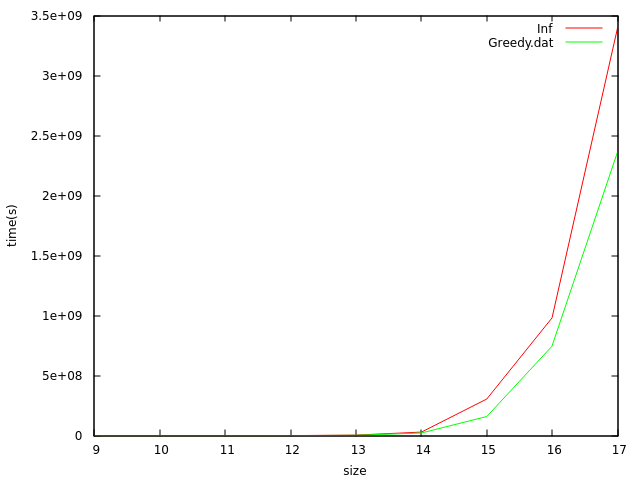
\includegraphics[width=0.8\textwidth]{ComparativaExploradosInf-Greedy.png}
				\caption{Gráfica comparativa de nodos explorados.}
				
			\end{figure}

			\vspace{2mm}

			\par
			En la gráfica anterior podemos observar cómo el disponer de una cota superior inicial más realista permite descartar muchas posibilidades desde el principio.

\newpage

			\par
			Como consecuencia, el factor de ramificación se reduce y, con él, el número de nodos que es necesario podar en fases posteriores de la ejecución. Esto se comprueba aquí:

			\vspace{2mm}

			\begin{figure}[h]

				\centering
				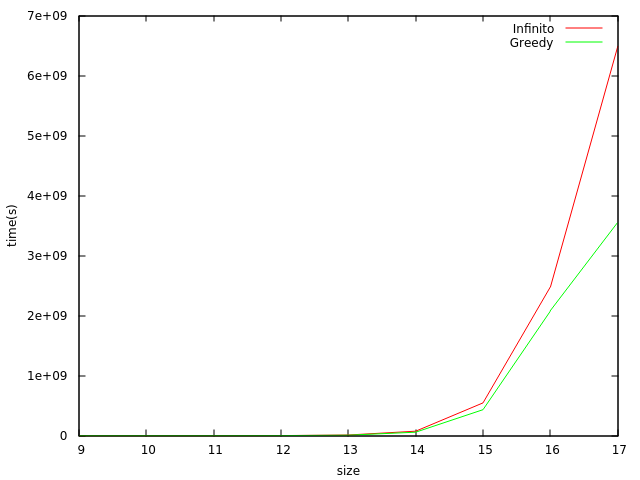
\includegraphics[width=0.8\textwidth]{ComparativaPodadosInf-Greedy.png}
				\caption{Gráfica comparativa de nodos podados.}
				
			\end{figure}

\newpage

	\section{Comparativa entre \textit{Ramificación y Poda} y \textit{Backtracking}.}

		\par
		En este apartado vamos a comparar ambos algoritmos bajo las mismas condiciones según el tiempo consumido y el esfuerzo de exploración del espacio de búsqueda realizado. Para ello, se ha utilizado como criterio de poda la heurística 1 y como cota superior inicial una solución \textit{Greedy}; para más detalles sobre estos componentes, ver la \hyperlink{improvements}{\textbf{sección anterior}}.

		\par
		En primer lugar, presentamos los tiempos de ejecución de ambos algoritmos mediante una tabla y su gráfica asociada:

		\vspace{2mm}

		\begin{figure}[h]

			\centering

			\begin{tabular}{| >{\centering\arraybackslash}m{1in} | >{\centering\arraybackslash}m{1in} | >{\centering\arraybackslash}m{1in} |}

				\hline
				\textbf{Tamaño} & \textbf{Ramificación y Poda} & \textbf{Backtracking} \\
				\hline
				9 & 0.005936 & 0.004954 \\
				\hline
				10 & 0.025171 & 0.019709 \\
				\hline
				11 & 0.097976 & 0.079026 \\ 
				\hline
				12 & 0.40271 & 0.409318 \\
				\hline
				13 & 2.39737 & 2.62488 \\
				\hline
				14 & 15.5334 & 15.9302 \\
				\hline
				15 & 113.248 & 142.929 \\
				\hline
				16 & 507.988 & 553.935 \\
				\hline 
				17 & 1403.64 & 1732.71 \\
				\hline

			\end{tabular}
			\caption{Tiempos de ejecución de los dos algoritmos sobre subconjuntos de la instancia \textit{ulysses22}.}

		\end{figure}

		\begin{figure}[h]

			\centering
			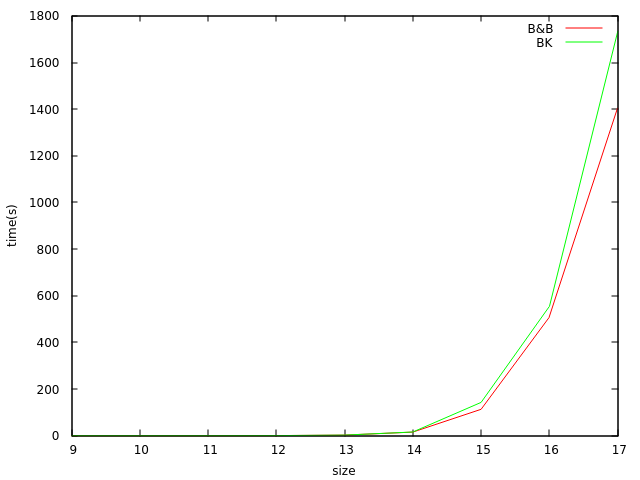
\includegraphics[width=0.7\textwidth]{ComparativaB&B-BK.png}
			\caption{Gráfica comparativa de tiempos de ejecución. Intel® Core™ i5-5200U CPU @ 2.20GHz.}
			
		\end{figure}

\newpage

		\par
		Sin embargo, el tiempo de ejecución no es el único dato relevante a la hora de comparar estas técnicas. Para ilustrar mejor las diferencias, podemos compararlas también según el número total de nodos explorados y el número de podas realizadas:
		
		\vspace{2mm}

		\begin{figure}[h]

			\centering

			\begin{tabular}{| >{\centering\arraybackslash}m{1in} | >{\centering\arraybackslash}m{1in} | >{\centering\arraybackslash}m{1in} | >{\centering\arraybackslash}m{1in} | >{\centering\arraybackslash}m{1in} |}

				\hline
				\multirow{3}{*}{\textbf{Tamaño}} & \multicolumn{2}{ c |}{Nodos explorados} & \multicolumn{2}{c |}{Podas realizadas} \\
				\cline{2-5}
				 & \textbf{Ramificación y Poda} & \textbf{Backtracking} & \textbf{Ramificación y Poda} & \textbf{Backtracking} \\
				\hline
				9 & 11835 & 24879 & 13931 & 11433 \\
				\hline
				10 & 46104 & 100544 & 68824 & 55162 \\
				\hline
				11 & 169904 & 386177 & 315454 & 239130 \\ 
				\hline
				12 & 658812 & 1883271 & 1411538 & 1230383 \\
				\hline
				13 & 3700596 & 11417664 & 8897596 & 7116013 \\
				\hline
				14 & 22759953 & 66055391 & 59114136 & 46618259 \\
				\hline
				15 & 159973208 & 555393772 & 433414136 & 396271023 \\
				\hline
				16 & 747710543 & 2551655421 & 2075155499 & 1541858327 \\
				\hline
				17 & 2362464162 & 3612963039 & 6545043838 & 3079201741 \\
				\hline

			\end{tabular}
			\caption{Otros datos relevantes de los dos algoritmos.}

		\end{figure}

		\par
		La diferencia en número de nodos explorados y podados se ve en las siguientes dos gráficas:

		\vspace{2mm}

		\begin{figure}[h]

			\centering
			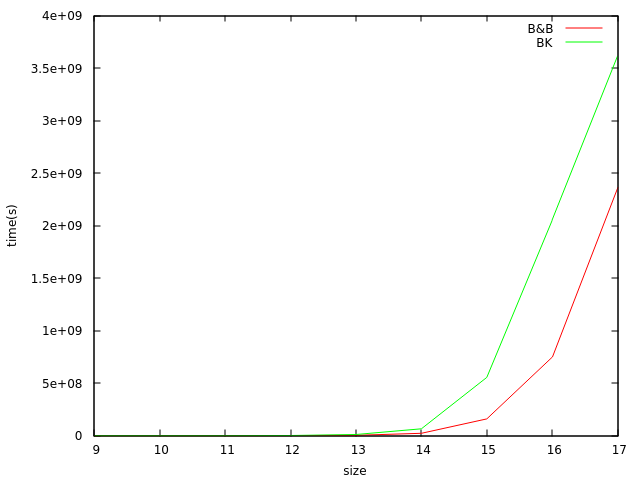
\includegraphics[width=0.75\textwidth]{ComparativaExploradosBk-B&B.png}
			\caption{Gráfica comparativa de nodos explorados.}
			
		\end{figure}

		\vspace{2mm}

		\par
		Como podemos observar, \textit{Ramificación y Poda} explora muchos menos nodos que \textit{Backtracking}.

\newpage

		\par
		Y, sin embargo, también es capaz de podar una mayor cantidad de nodos.

		\vspace{2mm}

		\begin{figure}[h]

			\centering
			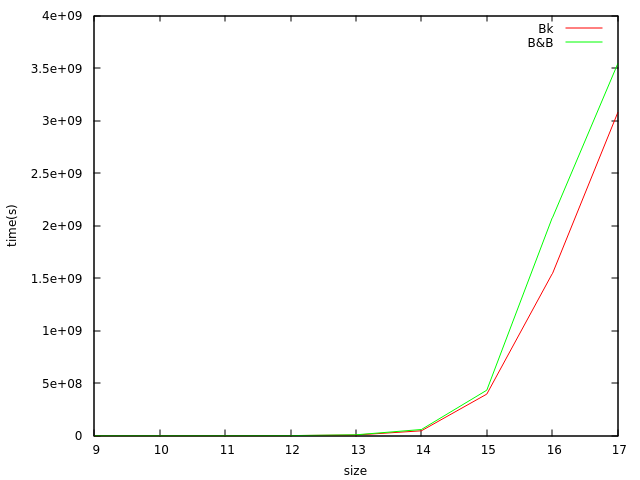
\includegraphics[width=0.75\textwidth]{ComparativaPodadosBk-B&B.png}
			\caption{Gráfica comparativa de nodos podados.}
			
		\end{figure}	

	\section{Conclusión.}

		\par
		A la vista de los resultados de la práctica, podemos decir que un técnica de \textit{Ramificación y Poda} es mejor que una técnica \textit{Backtracking} para resolver de forma óptima el problema del viajante de comercio, excepto en aquellos casos en los que la carga que supone manejar las estructuras de datos necesarias hace que \textit{Ramificación y Poda} emplee más tiempo en resolver el problema (esto sucede para volúmenes de datos pequeños).

		\par
		Es destacable también la elección de una buena heurística y la forma de determinar la cota superior inicial, ya que influyen de manera notable en la eficiencia del algoritmo. Cuanto más se ajusten ambas a la realidad, más eficiente será nuestro algoritmo.

		\par
		Otra forma de disminuir los tiempos de ejecución es la optimización del compilador. Esto nos ha permitido realizar pruebas con dimensiones un poco más grandes, por lo cual concluimos que es una opción a tener en cuenta.

		\par
		En cuanto a cuestiones de implementación, debemos tener cuidado a la hora de elegir la representación interna de los datos, puesto que, por ejemplo, un dato de tipo entero no es capaz de almacenar la suma de los nodos explorados o expandidos para volúmenes de datos considerables; en ese caso, sería necesario un tipo de dato con mayor capacidad. Asimismo, no hay que despreciar el orden de eficiencia del cálculo de la valoración optimista de cada nodo, puesto que es un cálculo que puede llegar a realizarse millones de veces y, por tanto, influye notablemente en el tiempo de ejecución del algoritmo.

\end{document}